%%% The main file. It contains definitions of basic parameters and includes all other parts.

%% Settings for single-side (simplex) printing
% Margins: left 40mm, right 25mm, top and bottom 25mm
% (but beware, LaTeX adds 1in implicitly)
\documentclass[12pt,a4paper]{report}
\setlength\textwidth{145mm}
\setlength\textheight{247mm}
\setlength\oddsidemargin{15mm}
\setlength\evensidemargin{15mm}
\setlength\topmargin{0mm}
\setlength\headsep{0mm}
\setlength\headheight{0mm}
% \openright makes the following text appear on a right-hand page
\let\openright=\clearpage

%% Settings for two-sided (duplex) printing
% \documentclass[12pt,a4paper,twoside,openright]{report}
% \setlength\textwidth{145mm}
% \setlength\textheight{247mm}
% \setlength\oddsidemargin{14.2mm}
% \setlength\evensidemargin{0mm}
% \setlength\topmargin{0mm}
% \setlength\headsep{0mm}
% \setlength\headheight{0mm}
% \let\openright=\cleardoublepage

%% Generate PDF/A-2u
\usepackage[a-2u]{pdfx}

%% Character encoding: usually latin2, cp1250 or utf8:
\usepackage[utf8]{inputenc}

%% Prefer Latin Modern fonts
\usepackage{lmodern}

%% Further useful packages (included in most LaTeX distributions)
\usepackage{amsmath}        % extensions for typesetting of math
\usepackage{amsfonts}       % math fonts
\usepackage{amsthm}         % theorems, definitions, etc.
\usepackage{bbding}         % various symbols (squares, asterisks, scissors, ...)
\usepackage{bm}             % boldface symbols (\bm)
\usepackage{graphicx}       % embedding of pictures
\usepackage{fancyvrb}       % improved verbatim environment
\usepackage{natbib}         % citation style AUTHOR (YEAR), or AUTHOR [NUMBER]
\usepackage[nottoc]{tocbibind} % makes sure that bibliography and the lists
			    % of figures/tables are included in the table
			    % of contents
\usepackage{dcolumn}        % improved alignment of table columns
\usepackage{booktabs}       % improved horizontal lines in tables
\usepackage{paralist}       % improved enumerate and itemize
\usepackage{xcolor}         % typesetting in color

%%% Basic information on the thesis

% Thesis title in English (exactly as in the formal assignment)
\def\ThesisTitle{Development and deployment of SaaS solution for logistics automation in e-commerce}

% Author of the thesis
\def\ThesisAuthor{Bc. Michal Půlpán}

% Year when the thesis is submitted
\def\YearSubmitted{2024}

% Name of the department or institute, where the work was officially assigned
% (according to the Organizational Structure of MFF UK in English,
% or a full name of a department outside MFF)
\def\Department{Department of Software Engineering}

% Is it a department (katedra), or an institute (ústav)?
\def\DeptType{Department}

% Thesis supervisor: name, surname and titles
\def\Supervisor{Mgr. Petr Škoda, Ph.D.}

% Supervisor's department (again according to Organizational structure of MFF)
\def\SupervisorsDepartment{Department of Software Engineering}

% Study programme and specialization
\def\StudyProgramme{Computer Science}
\def\StudyBranch{Software and Data Engineering (ISDP)}

% An optional dedication: you can thank whomever you wish (your supervisor,
% consultant, a person who lent the software, etc.)
\def\Dedication{%
Dedication.
}

% Abstract (recommended length around 80-200 words; this is not a copy of your thesis assignment!)
\def\Abstract{%
Abstract.
}

% 3 to 5 keywords (recommended), each enclosed in curly braces
\def\Keywords{%
{e-commerce} {logistics} {process automation} {web application} {software as a service}
}

%% The hyperref package for clickable links in PDF and also for storing
%% metadata to PDF (including the table of contents).
%% Most settings are pre-set by the pdfx package.
\hypersetup{unicode}
\hypersetup{breaklinks=true}

% Definitions of macros (see description inside)
%%% This file contains definitions of various useful macros and environments %%%
%%% Please add more macros here instead of cluttering other files with them. %%%

%%% Minor tweaks of style

% These macros employ a little dirty trick to convince LaTeX to typeset
% chapter headings sanely, without lots of empty space above them.
% Feel free to ignore.
\makeatletter
\def\@makechapterhead#1{
  {\parindent \z@ \raggedright \normalfont
   \Huge\bfseries \thechapter. #1
   \par\nobreak
   \vskip 20\p@
}}
\def\@makeschapterhead#1{
  {\parindent \z@ \raggedright \normalfont
   \Huge\bfseries #1
   \par\nobreak
   \vskip 20\p@
}}
\makeatother

% This macro defines a chapter, which is not numbered, but is included
% in the table of contents.
\def\chapwithtoc#1{
\chapter*{#1}
\addcontentsline{toc}{chapter}{#1}
}

% Draw black "slugs" whenever a line overflows, so that we can spot it easily.
\overfullrule=1mm

%%% Macros for definitions, theorems, claims, examples, ... (requires amsthm package)

\theoremstyle{plain}
\newtheorem{thm}{Theorem}
\newtheorem{lemma}[thm]{Lemma}
\newtheorem{claim}[thm]{Claim}

\theoremstyle{plain}
\newtheorem{defn}{Definition}

\theoremstyle{remark}
\newtheorem*{cor}{Corollary}
\newtheorem*{rem}{Remark}
\newtheorem*{example}{Example}

%%% An environment for proofs

\newenvironment{myproof}{
  \par\medskip\noindent
  \textit{Proof}.
}{
\newline
\rightline{$\qedsymbol$}
}

%%% An environment for typesetting of program code and input/output
%%% of programs. (Requires the fancyvrb package -- fancy verbatim.)

\DefineVerbatimEnvironment{code}{Verbatim}{fontsize=\small, frame=single}

%%% The field of all real and natural numbers
\newcommand{\R}{\mathbb{R}}
\newcommand{\N}{\mathbb{N}}

%%% Useful operators for statistics and probability
\DeclareMathOperator{\pr}{\textsf{P}}
\DeclareMathOperator{\E}{\textsf{E}\,}
\DeclareMathOperator{\var}{\textrm{var}}
\DeclareMathOperator{\sd}{\textrm{sd}}

%%% Transposition of a vector/matrix
\newcommand{\T}[1]{#1^\top}

%%% Various math goodies
\newcommand{\goto}{\rightarrow}
\newcommand{\gotop}{\stackrel{P}{\longrightarrow}}
\newcommand{\maon}[1]{o(n^{#1})}
\newcommand{\abs}[1]{\left|{#1}\right|}
\newcommand{\dint}{\int_0^\tau\!\!\int_0^\tau}
\newcommand{\isqr}[1]{\frac{1}{\sqrt{#1}}}

%%% Various table goodies
\newcommand{\pulrad}[1]{\raisebox{1.5ex}[0pt]{#1}}
\newcommand{\mc}[1]{\multicolumn{1}{c}{#1}}



\makeatletter
\newif\ifAC@uppercase@first
\def\Aclp#1{\AC@uppercase@firsttrue\aclp{#1}\AC@uppercase@firstfalse}
\def\AC@aclp#1{%
  \ifcsname fn@#1@PL\endcsname
    \ifAC@uppercase@first
      \expandafter\expandafter\expandafter\MakeUppercase\csname fn@#1@PL\endcsname
    \else
      \csname fn@#1@PL\endcsname
    \fi
  \else
    \AC@acl{#1}s
  \fi 
}
\edef\AC@uppercase@write{\string\ifAC@uppercase@first\string\expandafter\string\MakeUppercase\string\fi\space}
\def\AC@acrodef#1[#2]#3{%
  \@bsphack
  \protected@write\@auxout{}{%
    \string\newacro{#1}[#2]{\AC@uppercase@write #3}%
  }\@esphack
}
\def\Acl#1{\AC@uppercase@firsttrue\acl{#1}\AC@uppercase@firstfalse}
\makeatother


% Title page and various mandatory informational pages
\begin{document}
%%% Title page of the thesis and other mandatory pages

%%% Title page of the thesis

\pagestyle{empty}
\hypersetup{pageanchor=false}
\begin{center}

\centerline{\mbox{
\includegraphics[width=166mm]{img/logo-en.pdf}}}

\vspace{-8mm}
\vfill

{\bf\Large MASTER THESIS}

\vfill

{\LARGE\ThesisAuthor}

\vspace{15mm}

{\LARGE\bfseries\ThesisTitle}

\vfill

\Department

\vfill

{
\centerline{\vbox{\halign{\hbox to 0.45\hsize{\hfil #}&\hskip 0.5em\parbox[t]{0.45\hsize}{\raggedright #}\cr
Supervisor of the master thesis:&\Supervisor \cr
\noalign{\vspace{2mm}}
Study programme:&\StudyProgramme \cr
\noalign{\vspace{2mm}}
%Study branch:&\StudyBranch \cr
}}}}

\vfill

% Zde doplňte rok
Prague \YearSubmitted

\end{center}

\newpage

%%% Here should be a bound sheet included -- a signed copy of the "master
%%% thesis assignment". This assignment is NOT a part of the electronic
%%% version of the thesis. DO NOT SCAN.

%%% A page with a solemn declaration to the master thesis

\openright
\hypersetup{pageanchor=true}
\pagestyle{plain}
\pagenumbering{roman}
\vglue 0pt plus 1fill

\noindent
I declare that I carried out this master thesis independently, and only with the cited
sources, literature and other professional sources. It has not been used to obtain another
or the same degree.

\medskip\noindent
I understand that my work relates to the rights and obligations under the Act No.~121/2000 Sb.,
the Copyright Act, as amended, in particular the fact that the Charles
University has the right to conclude a license agreement on the use of this
work as a school work pursuant to Section 60 subsection 1 of the Copyright~Act.

\vspace{10mm}

\hbox{\hbox to 0.5\hsize{%
In \hbox to 6em{\dotfill} date \hbox to 6em{\dotfill}
\hss}\hbox to 0.5\hsize{\dotfill\quad}}
\smallskip
\hbox{\hbox to 0.5\hsize{}\hbox to 0.5\hsize{\hfil Author's signature\hfil}}

\vspace{20mm}
\newpage

%%% Dedication

\openright

\noindent
\Dedication

\newpage

%%% Mandatory information page of the thesis

\openright

%\vbox to 0.5\vsize{
%\setlength\parindent{0mm}
%\setlength\parskip{5mm}


\vtop to 0.5\vsize{
\setlength\parindent{0mm}
\setlength\parskip{5mm}

Title:
\ThesisTitle

Author:
\ThesisAuthor

\DeptType:
\Department

Supervisor:
\Supervisor, \SupervisorsDepartment

Abstract:
\Abstract

Keywords:
\Keywords

\vfil
}
\newpage

\vtop to 0.5\vsize{
\setlength\parindent{0mm}
\setlength\parskip{5mm}

Název práce:
\ThesisTitleCZ

Autor:
\ThesisAuthor

\DeptTypeCZ:
\DepartmentCZ

Vedoucí práce:
\Supervisor, \SupervisorsDepartmentCZ

Abstrakt:
\AbstractCZ

Klíčová slova:
{\def\sep{\unskip, }\KeywordsCZ}

\vfil
}
%\vss

\newpage

\openright
\pagestyle{plain}
\pagenumbering{arabic}
\setcounter{page}{1}


%%% A page with automatically generated table of contents of the master thesis

\tableofcontents

%%% Each chapter is kept in a separate file
\chapter*{Introduction}
\label{chap:introduction}
\addcontentsline{toc}{chapter}{Introduction}
% General introduction to the problem -> ecommerce, communication with shipping carriers
% Why is it hard 
In recent years, e-Commerce has experienced rapid growth, changing the retail environment across the globe.
This trend, strongly reflected in the Czech Republic, has placed online shopping not only as an alternative to physical retail, but also often as the preferred shopping channel for a wide demographic.
The rapid rise of e-Commerce in the Czech Republic, along with the broader Central and Eastern European region, introduces competitive challenges and opportunities.
According to the \cite{ApekEcommerceStudy2023} E-commerce Study 2023 by Czech Association for Electronic Commerce (\ac{APEK}), the Czech market was worth about \$8 billion in 2023 with 61\% of the Czech Internet population (15 +) shopping at least once a month online.
As more consumers turn to online shopping, the market has become saturated with the large number of vendors that demand attention with significant marketing budgets.
This situation requires brands to do more than just offer products; they must present distinct identities, maintain brand values, and establish deeper connections with their customers.
Brands must aim to differentiate themselves, turning the focus towards building a recognisable brand presence while keeping up with customer care. 

The competitive core of e-Commerce enforces brands to refine their strategies. In this context, the battle is not just about sales, but also about becoming the go-to-shop within the product domain. 
%This requires an innovative approach to enhance the shopping experience, making it not only seamless and convenient, but also memorable and distinctive. 
Ogunmola and Kumar \cite{ecommerce-research-models} emphasise that the growing competitive environment in online retail forces brands to continuously innovate, especially to improve the shopping experience to differentiate themselves and achieve a dominant position in the market.
Brand must wisely think about every touch point, from website quality to user interface, user experience, customer service, and logistics, as an opportunity to boost brand awareness and values.

The logistical aspect of e-Commerce, often seen as a backend operation, has come to the forefront as an important part of customer satisfaction and brand differentiation.
Efficiency in order processing, reliability in shipping, and transparency in delivery updates are now increasingly important in the customer experience.
In today's fast digital world, consumer's patience for slow order processing has significantly decreased.
According to the mentioned study by \ac{APEK} in September 2023, a growing number of customers report that transparency in delivery times and fast order processing are among their main considerations when choosing between two vendors.
This highlights a clear trend: Customers are willing to pay a premium for the assurance of a faster and more transparent delivery.
This shift brings a new challenge to e-Commerce businesses; slow order processing is no longer just a logistical issue but is directly related to customer retention and brand loyalty.
With that said, it is clear that the customer paying more attention to the delivery time of their order, will be likely to appreciate continuous updates of their order status in a user interface similar to the e-Commerce store they purchased from.
This presents a problem that many e-Commerce platforms and retailers are dealing with: how to streamline their logistic operations to meet the demands of modern consumers.

The solution proposed in this thesis aims to address these needs by creating a simple-to-use platform designed for dispatching orders to the shipping carriers, seamlessly sending data to the carriers, printing shipping labels, and updating order statuses.
In addition, this platform will serve as a new marketing communication channel, offering a branded parcel tracking experience.

To ensure the applicability of the platform in real-world scenarios, this project will also include the implementation of a connector for SAP Business One. This integration will enable the seamless exchange of data between third-party software and SAP Business One. The platform will be tested in a company that operates in both the \ac{B2B} and \ac{B2C} segments of the fashion e-Commerce industry, handling more than 100 packages per day. 
This environment presents an ideal setting for evaluating the platform's capabilities.


\subsection*{Motivation}
\label{subsec:motivation}
% Motivation -> how does the proccess generally look like and how I'm going to make it more efficient
Process of dispatching orders, communicating with shipping carriers, and providing customers with timely update is full of inefficiency and challenges.
Traditionally, these operations involve various manual interventions, leading to delays and errors that directly impact customer satisfaction and brand loyalty.
In an era where consumers value speed, it is not viable to manually upload data set to the carriers web interface and then request shipping labels if everything goes well. 
For a company that cooperates with multiple shipping carriers, this process becomes quickly unsustainable.
It has to be automatic with direct feedback of data errors and import problems. For example, if the shipping address is not valid or if the carrier raises any other error with the provided data set or its own service.
Having said that, each carrier is an isolated company without any unification when it comes to the data they accept and provide.
Bridging the gap between the communication interface of each carrier and generalising parcel shipping statuses quickly becomes a very appreciated task. 
As a result, businesses can seamlessly integrate new shipping carriers without being bogged down by the specific implementation details and the varying data formats each carrier uses.
%because programmers need to read only single documentation and understand only one data format without having to care about any implementation details and specifics.

%When a company collects the data obtained from its shipping carriers, it is also important to use it.
When a company collects data from its shipping carriers, it is important to utilise this information.
Leveraging such data not only streamlines operations but also provides a competitive advantage by improving decision making and improving customer satisfaction and brand recognition.
We will use this opportunity to present the tracking data with a company branding to increase brand awareness and create a new and unexplored marketing channel that customers are not used to and therefore resistant to.

The goal is to transform logistics from a potential pain point into a competitive advantage for e-Commerce businesses, thus not only meeting but exceeding customer expectations by providing them with a branded tracking page and automatic e-mail notifications with branding.

\subsection*{Project goals}
\label{subsec:project-goals}
% Project goals
The project is driven by a set of clear goals designed to address the challenges identified in the e-Commerce logistics domain and the software development itself:
\begin{enumerate}[label=\bfseries G\arabic*:,leftmargin=*]
    \item \textbf{Streamline logistics operations:} Develop a platform that simplifies the process of dispatching orders to shipping carriers, automating data exchange, and minimizing need for manual intervention.
    \item \textbf{Modern cloud based multi-tenant solution:} Create application with multi-tenant architecture allowing it to be used by multiple companies deployed to the cloud with automated integration and deployment. 
    \item \textbf{Create branded shipping customer experience:} Introduce a new marketing communication platform using the data collected from the shipping carrier that allowed each company to specify custom branding for the parcel tracking page and parcel status notification emails.
    \item \textbf{Integration with existing systems:} Develop a solution that can be easily integrated with existing businesses' system.
    \item \textbf{Validate in a real-world setting with SAP Business One integration:} Test the platform in a live e-Commerce environment, handling a significant volume of orders in daily operations.
\end{enumerate}

\subsection*{Solution overview}
\label{subsec:solution-overview}
% Saas
% Deployment
% SAP Business One integration
% Real-life usage in the daily operation of an B2C and B2B focused company
The proposed solution is a Software as a Service (\ac{SaaS}) platform designed to modernize and simplify e-Commerce order data dispatch logistics. As its core, the platform will facilitate order dispatching to the shipping carrier, label printing, and periodic updates of order statuses. 

The entire code base will use continuous integration (\ac{CI}) practices and automatic deployment (\ac{CD}) to the Amazon Web Services (\ac{AWS}) ensuring high availability, security, and fast response times with resource scaling based on traffic.

The platform's user interface will be intuitive, well-documented, and easy to use, requiring minimal training for staff, and will provide customisable options for businesses to maintain their brand identity throughout the customer's post-purchase journey.
The branded tracking pages and notification emails are not just an enhancement of the logistics process; it is a redefinition of how businesses communicate with their customers, transforming every shipment into opportunity for engagement and brand reinforcement.

The testing and validation of the platform will take place in a company operating in both \ac{B2B} and \ac{B2C} segments of the fashion e-Commerce industry, dealing with more than 100 orders daily and running an instance of SAP Business One with which the platform will have to exchange data. 
This real-life usage will provide thorough testing of the platform and provides valuable insight.

% 

This thesis is organised to comprehensively address the dual aspects of exploitation and exploration within software development, together with the challenges of solution analysis, implementation, and integration encountered in working with SAP Business One.

\begin{itemize}
    \item \textbf{Related Work \ref{chap:related-work}:} Reviews industry options in the sector and discusses project objectives.
    \item \textbf{Analysis \ref{chap:analysis}:} It represents the actual work process within a given problem domain with the result of functional and non-functional requirements for a proposed platform.
    \item \textbf{Architecture \ref{chap:architectural-design}:} Outlines the architectural design of the proposed solution, describing its components and their interactions.
    \item \textbf{Technical design \ref{chap:technical-design}:} Describes the technical specifications and design considerations for creating a robust logistics platform.
    \item \textbf{Implementation \ref{chap:implementation}:} Details the development process of the logistics platform, including coding methodologies and software engineering practices.
    \item \textbf{Deployment \ref{chap:deployment}:} Explains the deployment strategy for the SaaS platform, including cloud hosting and service provisioning on Amazon Web Services.
    \item \textbf{SAP Integration \ref{chap:integrating-sap-b1}:} Discusses and presents the integration with SAP Business One, focusing on development of an application for direct data exchange with the ERP system. 
    \item \textbf{Evaluation \ref{chap:evaluation}:} Covers the evaluation used for validation the functionality and performance of the platform in real-world day-to-day business setting.
\end{itemize}
\chapter{Related work}
\label{chap:related-work}
% brief intorduction of the purpose of this chapter
% importance of understanding these works in the context of this project
This chapter dives into the overview of existing solutions within the scope of parcel logistics in the dispatch process, generating labels, and shipment tracking, with a focus on the Czech market.
Understanding these projects and their limitations helps us to understand the market gap that this project is filling.
Particularly in offering a cloud-based multi-tenant solution integrating customised tracking page and email notifications for recipients.
The overview underscores the importance of innovating beyond current offerings, which primarily lack features such as a simple dashboard for data viewing, custom tracking pages for improved customer communication, and automated email notifications.

\section{Related projects}
\label{sec:related-projects}
% boundaries of Czech environment and usage of local carriers - PPL, Packeta, Česká Pošta
% None of those implementing custom tracking page for customer communication 
% None of those implement auto e-mail sender to customer
% None of these is in cloud serving working as a multi tenant solution that customer doesn't have to care about

Projects handling data communication with carriers are, of course, heavily biased with the demographics they are targeting. 
Although the process is usually very similar, shipping companies and customers with their e-Commerce platforms or \ac{ERP} solutions are different.
Hence, we will limit ourselves to the Czech logistics environment, where several systems facilitate the integration with local carriers. However, these solutions often fall short in several areas:
\begin{itemize}
    \item None operates as a cloud-based multi-tenant solution that offers the business a hassle-free platform for their logistic needs without the necessity for in-house infrastructure or maintenance.
    \item Usually, they require a distinct approach and data model for different carriers. This makes it more difficult to integrate.
    \item They typically do not provide a custom tracking page for end-to-end customer communication, missing an opportunity to enhance the customer experience with a branded informative user interface.
\end{itemize}

Let us take a look at some options available in the Czech market.

\subsection{Balíkobot.cz}
\label{subsec:balikobot}
% integration directly into the ERP/ecommerce system
% no possibility to edit parcels outside of the ERP
% offloading processes from ERP
% SAP is fairly small and hardly accessible from the "outside" so it's not a great option
% usually doesn't directly implement data structure of the ERP
Offers integration directly into \ac{ERP}/e-Commerce systems, however lacking the flexibility to modify parcels outside of these systems.
Requiring that the user using this software is able to modify the source data in \ac{ERP} might be a strong limitation.
The next limitation might be the label format provided by Balíkobot.cz.
This solution generates its own layout of labels, validated by the carrier, of course, but sometimes a different layout might lead to inefficiency or even errors at the sorting centres or when loaded to the delivery vehicle.
On the other hand, the amount of integrated carriers and \ac{ERP} integrations makes Balikobot really easy to start using,
Overall, Balíkobot is definitely a considerable solution, but being integrated directly into the \ac{ERP} makes it a bit slow to use and is usually inaccessible from outside of the company network when needed.

However, it deals only with company processes, not with customer communication and presentation.

\subsection{LabelPrinter.cz}
\label{subsec:labelprinter}
% on premise windows service run at client
LabelPrinter, as name suggests, is meant for a label printing and data transfer. Similarly to Balíkobot, LabelPrinter only works as a warehouse software meant purely for the data transfer from company to carrier.
Additionally, it operates only as an on-premise Windows service runtime at the client's computer. 
This approach requires local infrastructure and maintenance, potentially increasing operational overhead in small to medium-sized enterprises, limiting scalability and accessibility.

% Zminit inhouse solution nebo to nechat byt??

\section{Addressing the shortcomings of existing solutions}
\label{sec:addressing-shortcoming-existing-solutions}
% - Abstract data model allowing for unified data format sent to the software
%- Dashboard with data overview seeing all the errors and direct label/consignment list printing accessible from outside network not beeing hosted locally
%- Unification of parcel statuses into few statuses only so that the user doesn't have differentiate between different carriers and translate statuses for their purpose
%- Branded parcel tracking page
%- Branded e-mail tracking notification
%- Not having to care about the deployment
%- Role based access for users
%- Having multiple projects with different carrier API credentials and settings

Problems of data communication with carriers present numerous challenges with existing solutions, particularly in their ability to scale and offer a seamless user experience across different carriers.
This project confronts these issues, presenting a new approach to the landscape of automation logistic expedition and post-purchase experience.

\subsection{Unified data model}
Existing solutions often lack a unified approach to data handling, which complicates integration with different carriers. 
This solution introduces a unified data model normalising data formats across all carriers, simplifying the integration, leaving the complexity of understanding different models to the project itself.

\subsection{Centralized dashboard}
Absence of a user-friendly dashboard in existing systems makes monitoring and managing shipments inconvenient, since most of it is left to the existing \ac{ERP} which is usually not made to handle logistics data.
Providing a modern web application with a dashboard accessible from anywhere brings a great competitive advantage and improves the user experience. 
With an overview of all data sent and retrieved from carriers and direct functionalities for label and consignment list printing, the user does not have to use any other interface when working with parcels.

\subsection{Parcel status unification}
The set of parcel statuses provided by the carriers is, of course, very distinct. Every carrier API is different; hence, it provides different data and communicates in a different way.
Consolidation of various statuses into a standardised set, allowing users to easily understand and manage the shipments without getting lost in carrier-specific environments.

\subsection{Branded tracking and notifications}
Enhancing post-purchase communication is often overlooked.
Businesses usually leave this channel to the third party (carrier) and focus on pre-purchase marketing, which is usually, in a digital marketing, standard \ac{PPC} adverts. 
However, as this segment becomes more regulated, some customers are difficult to approach.
Smartly communicating with a customer, when the most important part of the purchase is happening, could be a key to greater brand recall in today's advertising overload. 

\subsection{Simplified integration}
The technical challenges and costs of implementing and installing a software solution in premise might act as a barrier to many businesses. 
The cloud-based solution eliminates these obstructions.

\subsection{Role-based access control}
Security demands tailored access controls.
Implementing role-based access improves security and ensures that users have the appropriate permissions for their role.

\subsection{Versatile carrier communication}
Businesses often work with multiple shipping carriers with different contracts and settings. 
For example, each warehouse might require a different contract with the carrier when it is in a different region.
This can be difficult to manage. 
Hence, it is necessary to implement a solution that can manage multiple locations (projects) in one profile with different carrier API credentials and settings while distinguishing between shipments and users from different locations.




\chapter{Analysis}
\label{chap:analysis}
% recap of introduction - motiovation, goals + related work
% brief intorduction of the purpose of chapter
After framing context of the platform by presenting both motivation and goals with previewing related solutions, we take a closer look at the overall analysis for our software.
The purpose is to present the requirements placed on the system, primarily determined by the standard ordering process in the eCommerce sector.
In addition, the requirements resulting from the planned test deployment will be presented.

 %The purpose is to present and understand the order dispatch process flow and the practical implications of implementing and testing this solution within a real-world company environment.
And also to define the specific requirements that will guide the development of the platform.
This analysis is the foundation for a solution that not only meets technical specifications but also addresses practical business needs within a logistics sector and day-to-day usage.

This chapter will begin with a necessary introduction to the order dispatch process \ref{sec:order-dispatching-process}. 
Understanding this process is necessary to frame the context in which the entire system operates and in which users operate.
Then, after understanding the context, in the \ref{sec:real-world-applicability} section, an approach to testing the system will be presented, both from both the integration and user perspective.
Finally, after defining the environment in which the system is set and a way to verify the functionality, we can go to the \ref{sec:requirements} section.
This section will present the functional and non-functional requirements on the system.

% 



\section{Order dispatching process}
\label{sec:order-dispatching-process}
% describe how orders are processed from ordering online, to SAP Draft objects, to SAP order objects to packing list to finally passing to the shipping company and printing label with consignment list
This section dives into the general life-cycle of an order from the moment it is placed to the final delivery.
We will take into account the most simple and straightforward approach, which is usually the starting point for many companies and warehouses.
Defining this process helps to understand weaknesses and identify opportunities for automation and efficiency improvements.
Suppose a customer of a company is shopping in an e-Commerce store:

\begin{figure}[H]\centering
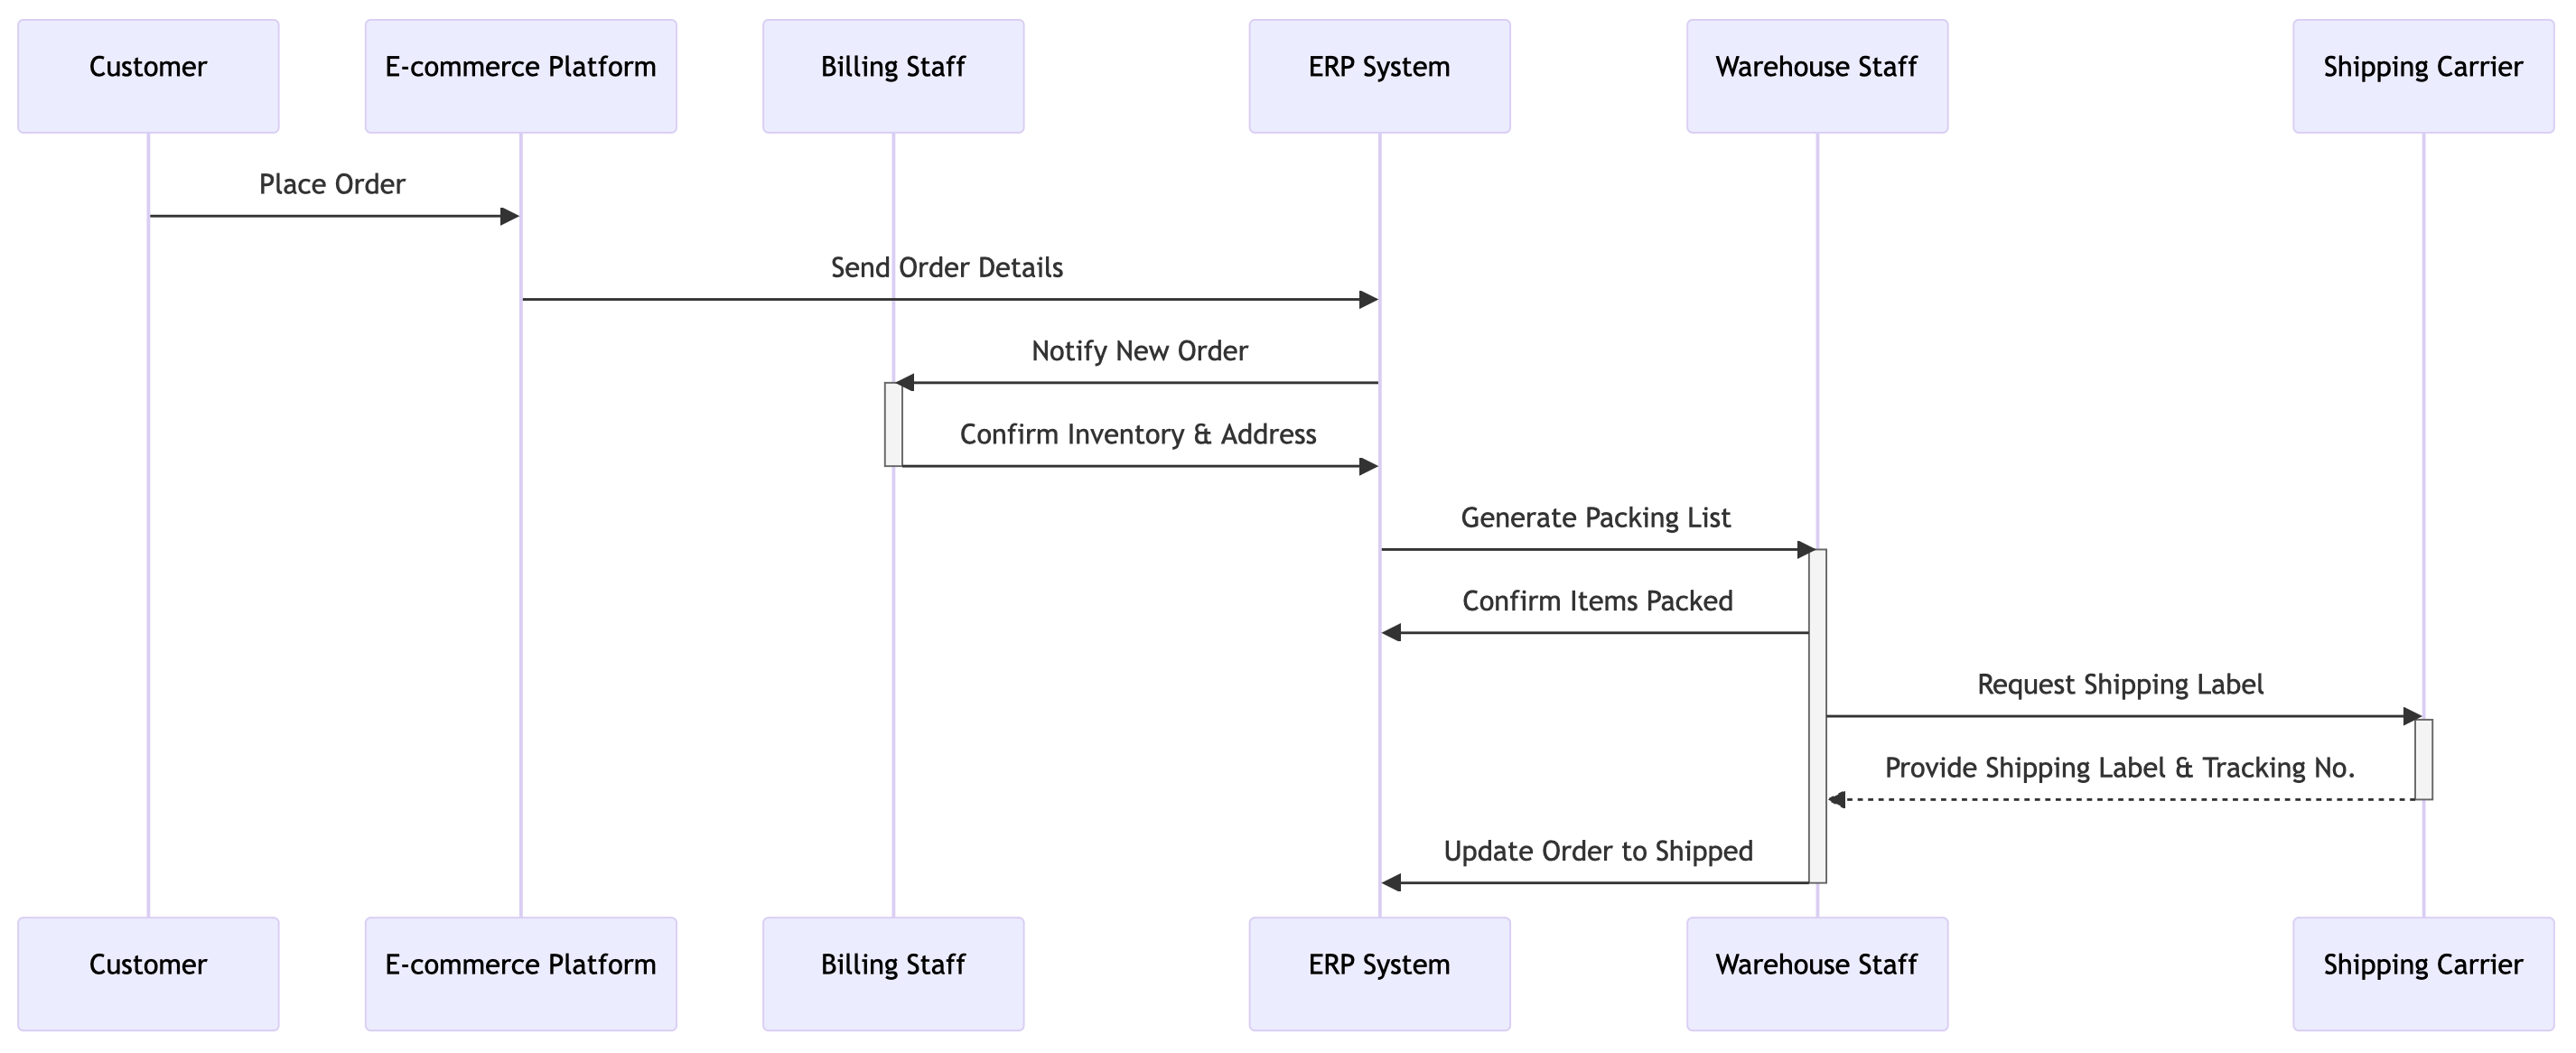
\includegraphics[width=140mm]{img/chap02/fig_proces_sequence_diagram_highres.png}
\caption{Sequence diagram of order dispatching process}
\label{img02:order-dispatch-process}
\end{figure}

%\begin{figure}[H]
%\centerline{\includesvg[width=140mm]{img/chap02/fig_proces_sequence_diagram.svg}}
%\caption{Sequence diagram of order dispatching process}
%\label{img02:order-dispatch-process}
%\end{figure}

\begin{enumerate}
    \item \textbf{Order placement:} Customer completes the checkout process with the shipping details and preferred shipping method. Order information is saved in the e-Commerce platform's database.
    \item \textbf{Order transfer to \ac{ERP}:} The order details are automatically transferred to the \ac{ERP} system. This transfer can occur at scheduled intervals or automatically, depending on the integration setup between the e-Commerce platform and the \ac{ERP}.
    \item \textbf{Order confirmation and inventory check:} The operator of the ERP system in the billing department processes the order with the validation of the shipping address and confirms the order.
    \item \textbf{Packing list and invoice generation:} Once the shipment is confirmed, the \ac{ERP} system generates a packing list that details the items to be shipped. At the same time, an order invoice is created.
    \item \textbf{Uploading shipments data:} With the items collected and packed, the next step involves generating a shipping label. Order data, including recipient information and insurance, are exported from \ac{ERP} to the format accepted by the carrier and uploaded to the carrier interface to retrieve the tracking number for each order.
    \item \textbf{Synchronizing tracking number with \ac{ERP}:} The list of selected orders in \ac{ERP} is altered with the tracking number retrieved from the carrier.
    \item \textbf{Shipping label and consignment list printing:} After orders receive tracking numbers, the shipping labels and the consignment list are downloaded from the carrier interface. The labels are then affixed to the consignments.
    \item \textbf{Shipment dispatch:} Shipments are handed over to the shipping company courier after signing the consignment list as a confirmation of receipt. 
    \item \textbf{Updating status and controlling delivery:} The list of parcel statuses is manually downloaded from the shipping company interface and uploaded to the \ac{ERP} system
\end{enumerate}


After a brief introduction to the process, we can see that points 5-9 are quite challenging.
Since the company may be working with multiple carriers at the same time, we get into a situation where the operator has to repeat these points for each carrier, making the process unsustainable and very time-consuming.
Not to mention that the company has to adapt to each carrier and create data exports and imports for each carrier separately.
In addition, the process of updating shipments is very complex and prone to errors.
For a visualisation using the sequence diagram, refer to \ref{img02:order-dispatch-process}.


% mermaid seq. diagram

%sequenceDiagram
%    participant Customer as Customer
%    participant ECommerce as E-commerce Platform
%    participant Billing as Billing Staff
%    participant ERP as ERP System
%    participant Warehouse as Warehouse Staff
%    participant Shipping as Shipping Carrier

%    Customer->>ECommerce: Place Order
%    ECommerce->>ERP: Send Order Details
%    ERP->>Billing: Notify New Order
%    activate Billing
%    Billing->>ERP: Confirm Inventory & Address
%    deactivate Billing
%    ERP->>Warehouse: Generate Packing List
%    activate Warehouse
%    Warehouse->>ERP: Confirm Items Packed
%    Warehouse->>Shipping: Request Shipping Label
%    activate Shipping
%    Shipping-->>Warehouse: Provide Shipping Label & Tracking No.
%    deactivate Shipping
%    Warehouse->>ERP: Update Order to Shipped
%    deactivate Warehouse



\section{Real-world applicability}
\label{sec:real-world-applicability}
% briefly note that the solution will be integrated and tested in the operating company
% it means for us, that we have to do implementation of three operating shipping carriers in the Czech republic (Ceska Posta, PPL, Packeta) so that company can seamlessly transtion + SAP integrations (so that the data can be stored in SAP for internal purposes and mark orders as shipped).
Platofrm's real-world applicability will be verified through integration and testing within an operating company.
Practical implementation will focus on incorporating three major shipping carriers in the Czech republic - Česká Pošta, PPL, and Packeta - to allow the company to make a seamless transition to use the platform.
This means that the platform will gain three carrier implementations with testing to offer to the rest of the user base.
Together with testing integration capabilities with external systems, namely \gls{sapb1}, it will be necessary to create a connector module presented in chapter \ref{chap:integrating-sap-b1}.

\section{Requirements}
\label{sec:requirements}
% intro, requirements (ref https://engineering.futureuniversity.com/BOOKS%20FOR%20IT/Software-Engineering-9th-Edition-by-Ian-Sommerville.pdf) with descriptiion of what's functional/nonfunctional requirement 
This section introduces the concept of software requirements.
In general, requirements are descriptions of the system's functionalities and what it should do while reflecting the needs of actors.
Requirements can be classified into two groups \cite{sommervilleSW}:
\begin{enumerate}
    \item \textit{Functional requirements:} describes how the system should react to particular inputs and how the system should behave in particular situations.
    \item \textit{Non-functional requirements:} constraints on the services of functions by the system. Including development process constraints and constraints defined by some standards. Non-functional requirements often apply to the system as a whole, rather than individual features.
\end{enumerate}
%For a better description, we will define the three actors used in the requirements later.
The whole system has three expected user roles:
\label{sec:requirements-actors}
\begin{enumerate}
    \item \textbf{Operator:} Role attributed to individuals employed by the company, interacting with the platform through its user interface. 
    \item \textbf{Developer:} Individual in this role utilises the platform's API for developing third-party integration.
    \item \textbf{Customer:} This role represents the end recipients who are waiting for the packages dispatched by the company using the platform.
\end{enumerate}

\begin{figure}[H]\centering
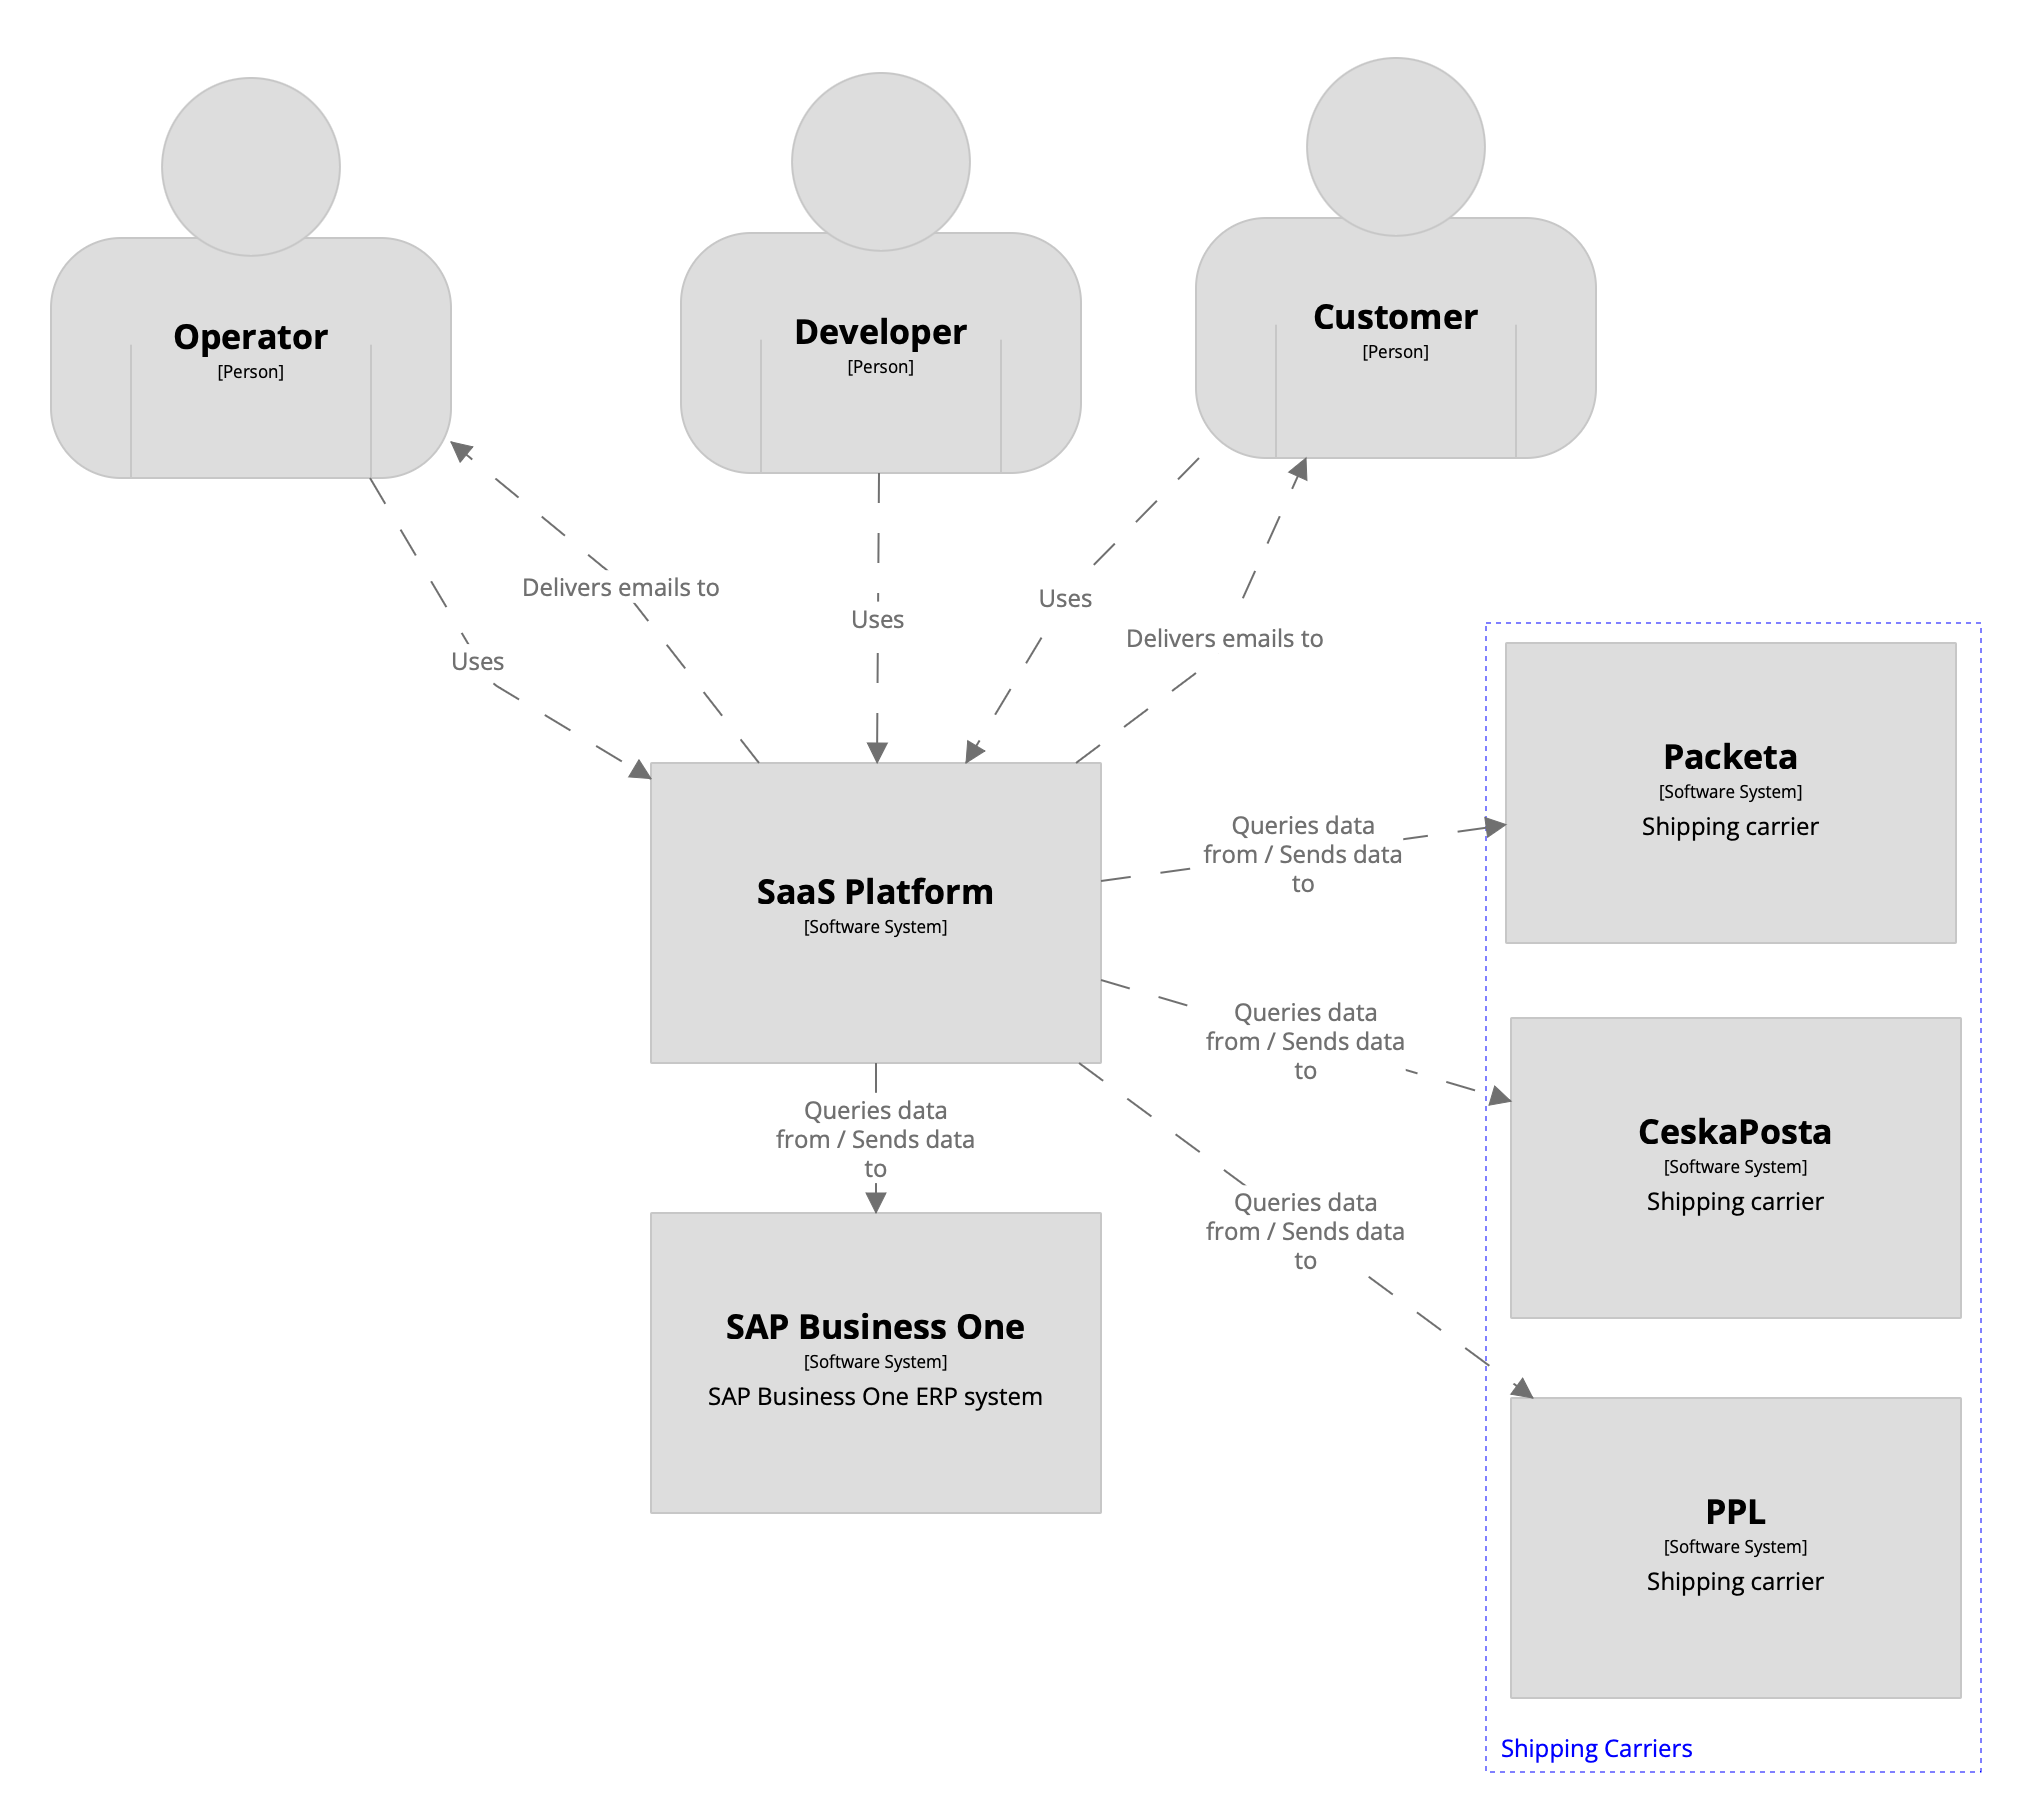
\includegraphics[width=140mm]{img/chap02/fig_system_context.png}
\caption{C4 diagram with system context}
\label{img02:analysis.system-context}
\end{figure}

To provide context, the platform operates as a \ac{SaaS} model and involves three key actors. We will demonstrate integration capabilities using \gls{sapb1}, along with production integration with three carriers: Packeta, PPL, and Česká Pošta. For a visual representation of the system context, refer to Figure \ref{img02:analysis.system-context}.

\subsection{Functional Requirements}
\label{subsec:functional-requirements}
% functions of the software itself and behaviour in given situations

%After researching the related work from chapter \ref{chap:related-work} and looking into the process - see section \ref{sec:order-dispatching-process}, a rough list of requirements was created based on information that can be freely obtained (for example, just from documentation and technical descriptions of existing solutions).
After reviewing the related work presented in Chapter \ref{chap:related-work} and analysing the process detailed in Section \ref{sec:order-dispatching-process}, an initial set of requirements was created.
These were primarily derived from readily available information, such as documentation and technical descriptions of existing solutions."

The whole list was then discussed with the company management (including IT and marketing) where the platform will be deployed for testing; see Section \ref{sec:real-world-applicability}. 
At the same time, the requirements were continuously communicated to the company's warehouse staff, who are considered as \textbf{operators} described in \ref{sec:requirements-actors} and will use the platform to get an overview of the processes and various situations that occur regularly and irregularly.

This newly acquired information provided the opportunity to design the requirements so that it would fit perfectly into the company's daily operations. 
The requirements were then slightly modified according to our own requirements for the platform, such as the limitation to the possibility of using one instance by multiple users, i.e. the platform should be designed as Software as a Service.


%\pointedenum\begin{enumerate}[\bfseries {FR}1{:}]
\begin{enumerate}[label=\bfseries FR\arabic*:,leftmargin=*]
    \item Operators can sign up and verify their accounts using a verification code sent to their provided email address.
    \item Operators can change password to their accounts using a verification code sent to their provided email address.
    \item Operators can log into their accounts using valid credentials.
    \item Operators can switch the interface language between Czech and English.
    \item Operators can create multiple \glspl{project} within their account to manage data separately (e.g., for different warehouses or companies).
    \item Operators can select and work within a specific \gls{project}.
    \item Operators can rename any of their \glspl{project}.
    \item Operators can delete any of their \glspl{project}.
    \item Operators can configure a default shipper for all shipments within a\\ \gls{project}.
    \item Operators can configure settings for shipping carrier APIs, including authentication (e.g., tokens, IDs, secrets) and other required fields.
    \item Within each \gls{project}, operators can create multiple sellers to customise the location and branding of the tracking page and the email notifications.
    \item For each \gls{seller}, operators can set the name, localization, and branding elements such as logo, primary colour, contact information (URL, email, phone, store name), and social media links (Facebook, Instagram,\\ YouTube, TikTok). operators can also enable customer email notifications for specific parcel statuses.
    \item Operators can remove any \gls{seller} from a \gls{project}.
    \item Operators can enter edit mode of the \gls{seller}.
    \item In \gls{seller} edit mode, operators can switch views between web and email to preview customer-facing pages and emails.
    \item Operators can generate API access tokens for developers to use.
    \item Operators can switch between \glspl{project} to which they have access.
    \item The operator can invite other operators to the \glspl{project}.
    \item Operators can invite new operators to collaborate on \glspl{project}.
    \item \Gls{project} collaborators can be assigned different roles (Owner, Admin, Member) with varying levels of permissions.
    \item Operators can view a paginated list of all shipments.
    \item Operators can adjust the number of shipment items displayed per page.
    \item Operators can navigate through the shipment list pages (next or previous).
    \item Operators can easily identify shipments by carrier (using colour coding and names) and those created on the current day directly from the list.
    \item Operators can apply filters to search through shipments based on textual data (reference, email) using four criteria (equal to, contains, starts with, ends with), date-time data (creation date) using a range picker, and list types (carrier, status) selecting multiple values.
    \item Operators can select multiple shipments across carriers and perform bulk actions on the selected items.
    \item Operators can send shipment data to carriers for all selected bulk shipments.
    \item Operators can generate shipping labels for selected shipments.
    \item Operators can generate a consignment list for selected shipments.
    \item Operators can initiate the creation of a new shipment with a single click on the shipment list page.
    \item When creating a new shipment, operators can specify details such as recipient, insurance, payment method and amount, carrier, and carrier services.
    \item Operators can add multiple parcels to a single shipment.
    \item Operators can preview or delete shipments after they have been sent to the carrier.
    \item Operators can edit or delete shipments before they are sent to the carrier.
    \item The system will automatically update the status of the shipments.
    \item If allowed by the seller, a notification email is sent to the customer when the status of the package is updated.
    \item Developers can retrieve all \gls{project} shipments through the API.
    \item Developers can create or update individual or multiple shipments through the API.
    \item Developers can list all parcels from the \gls{project} via the API.
    \item Developers can retrieve labels for selected shipments through the API.
    \item Developers can initiate the sending of shipment data to carriers for selected shipments via the API.
    \item Customers can receive branded email notifications about updates in the status of the parcel when permitted by the \gls{seller}.
    \item Customers can view the tracking page, customised with the seller's branding, displaying the parcel statuses.
\end{enumerate}

\subsection{Nonfunctional Requirements}
\label{subsec:nonfunctional-requirements}
% quality attributes of the software
% Multi-tenant architecture
% Docs
% CI/CD
% Source code (formatting, conventions)
% support for multiple carriers
The non-functional requirements were shaped by understanding the broader operational context.
These requirements focus on the quality attributes of the platform.

\subsubsection{Usability}
The user interface should be intuitive, requiring minimal training for warehouse and billing staff.
The dashboard of the platform is designed primarily to be used with a mouse and keyboard on standard desktop screens, but should also support touch interactions for versatility.
In addition, the tracking page is optimised primarily for touch interactions on mobile phones to enhance accessibility and ease of use for customers on the go. 
Provide user documentation, including guides for key processes.


\subsubsection{Extensibility}
The system should be able to easily integrate new APIs of the shipping carriers according to user demands.
Any new carrier integration should be seamlessly incorporated into the existing system, ensuring that from a user's perspective, the interaction remains uniform across all carriers.
This means that the user can initiate shipping processes with a single action, regardless of the carrier, allowing the system to handle the specifics in the background.

\subsubsection{Scalability}
Design the system to scale effortlessly to accommodate increases in both user base and request volume. 
The deployment strategy should enable automatic scaling based on current load, ensuring consistent performance even during peak operational periods. 
This approach ensures that the system remains responsive and efficient as demand grows.

%The infrastructure should automatically adjust resources based on load, ensuring seamless performance during peak times.

\subsubsection{Maintainability}
%Use coding standards and best practices to ensure that the source code is clean and easy to maintain.
To ensure that the source code is clean and easy to maintain, we will adhere to recognised coding standards and best practices. 
Specifically, we will use the Airbnb coding standard, which is widely respected for maintaining high-quality code in JavaScript environments.
Furthermore, \gls{eslint} will be employed as a linting tool to automatically check for errors and enforce these standards consistently throughout the development team.
Use a \ac{CI}/\ac{CD} pipeline for simple deployment and minimal downtime. 

\subsubsection{Multi-tenancy}
The system must support a multi-tenant architecture, allowing multiple companies to use the service simultaneously while keeping their data isolated.

\subsubsection{Integration}
Offer an API that supports integration with external systems with clear documentation.
Authentication should be handled by generating a long-lived token.

\subsubsection{Customization}
Allow for easy user customisation, including branded tracking pages and email notifications, to maintain consistency with the brand identity.




\chapter{Architectural design}
\label{chap:architectural-design}
% overview of the project
% high level view of the project - Present a bird’s-eye view of the project architecture, highlighting key components and their interactions, add diagrams for clarity
% view of the project in the context of the ecommerce company - how the architecture aligns with the business goals and operational needs of the e-commerce company. Include considerations like scalability, maintainability, and security.
% view of the project in the context of the ecommerce customer -  how the architectural design impacts the customer experience. Focus on usability, performance, and reliability from the customer’s perspective
% multitenancy - definitive design considerations and implementation strategy for supporting multitenancy in the architecture. 
% serverless - role and benefits of serverless architecture in the project. Discuss how serverless components are utilized for scalability, cost-effectiveness, and operational efficiency.

The architecture of robust software is not just the description of the technology used in the development process; it is the blueprint of the project.
As we transition from the foundational requirements outlined in the previous chapter \ref{sec:requirements}, we can start designing the overall project.
This chapter aims to present a high-level architecture of how communication is orchestrated between all services and key components of the project.
As stated in \cite{sommervilleSW}, the establishment of a robust architecture in the early stages of development is the key.
Because while refactoring components due to minor changes of requirements in the life-cycle of the software is usually relatively easy, refactoring a system architecture is likely to be quite expensive.
The reader can intuitively find parallel between house architecture and software architecture. 
Injection of foundations, or making foundations more robust while house sits on them will always be much more expensive and certainly with more compromises than when building a new house with a proper foundations.

%Since we are building an application whose purpose is to live in the cloud, serve multiple tenants, send emails, and provide a front-end with graphical user interface, we can roughly estimate what the architecture will look like.
%We will definitely need an application providing the user interface, functionalities, or the business logic, and store somewhere user data.

Since we are developing a web application designed for cloud deployment, several key architectural components become essential to meet our goals.
The aim is to create a solution that not only serves multiple tenants within a single instance, but also manages to send emails reliably and provides an intuitive graphical interface.
Given these constraints, we can foresee the foundational structure of our architecture.

As the core, our architecture will comprise three principal components:
\begin{enumerate}
    \item \textbf{User Interface:} A user-friendly front-end that serves as the primary interaction poit for users and customers (see definition of actors in section \ref{sec:requirements-actors}). This component is essential for information presentation and user input.
    \item \textbf{Business Logic Layer:} The backbone of our platform, where the essential functionalities and operational logic reside. This layer will encapsulate all the rules needed to run the core processes of our service. From handling user requests to processing data and orchestrating email notifications.
    \item \textbf{Data Storage:} A database system designed to store, manage, and retrieve user data, as well as application-specific information. Given the multi-tenant nature of the platform, the database architecture will be designed to ensure data isolation, integrity, and security for each tenant.
\end{enumerate}

To visualise the high-level approach of the few previously mentioned components, we will use a diagram of layered architecture. 
It is an architectural approach to organise the system into layers with different orders. 
In our case, the layered architecture would look as visualised in Figure \ref{img03:layered_architecture_diagram}.

\begin{figure}[p]\centering
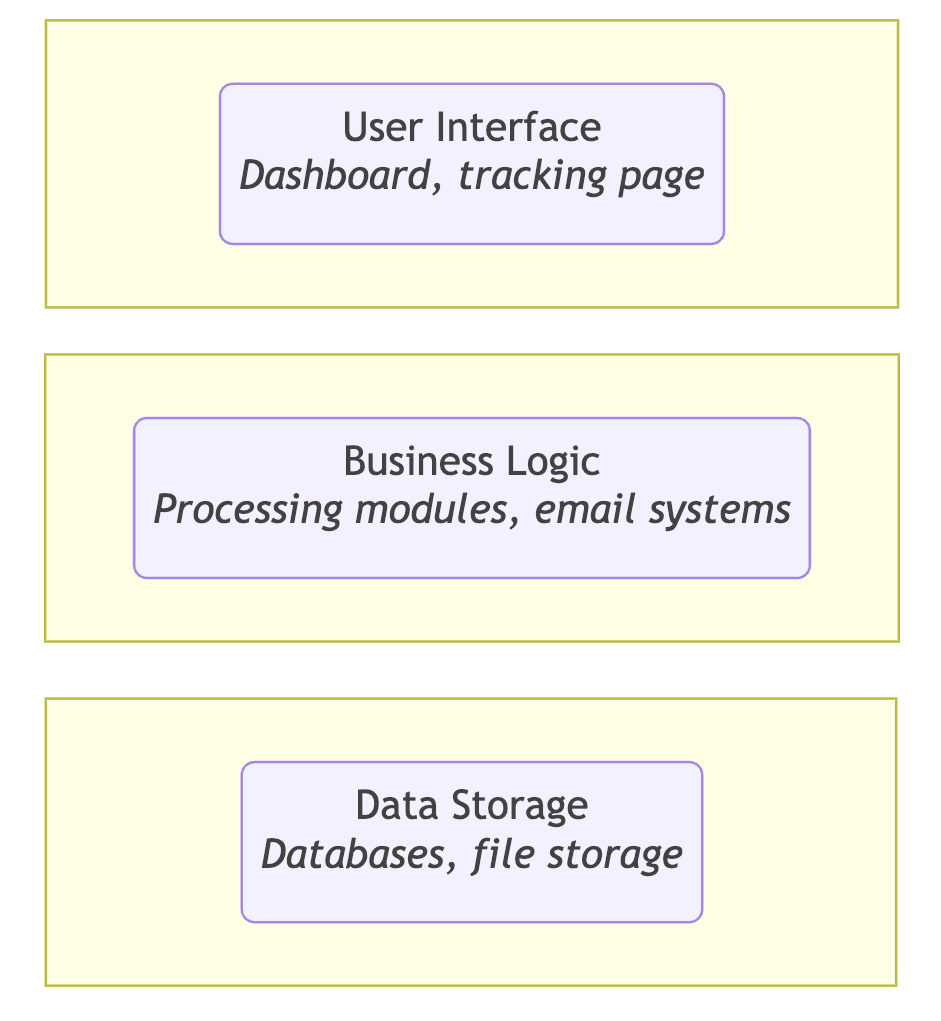
\includegraphics[width=140mm]{img/chap03/fig_layered_architecture_mermaid.png}
\caption{High-level layered architecture diagram}
\label{img03:layered_architecture_diagram}
\end{figure}

%graph TD;
%    UI[User Interface] --> BL[Business Logic];
%    BL --> DS[Data Storage];

%    subgraph UI_Layer[ ]
%        UI(User Interface<br><i>Dashboard, tracking page</i>)
%    end

%    subgraph BL_Layer[ ]
%        BL(Business Logic<br><i>Processing modules, email systems</i>)
%    end

%    subgraph DS_Layer[ ]
%        DS(Data Storage<br><i>Databases, file storage</i>)
%    end

%    style UI_Layer fill:#f9f,stroke:#333,stroke-width:2px
%    style BL_Layer fill:#ccf,stroke:#333,stroke-width:2px
%    style DS_Layer fill:#cfc,stroke:#333,stroke-width:2px

\section{Architectural Decisions}
\label{sec:architectural-decisions}
% Describe decisions made to desing the applicaiton
Before diving into the specifics of the application architecture, it is important to understand the foundational decisions that shape the overall architectural and implementation design of the platform.
These decisions are mainly influenced by non-functional requirements found in section \ref{subsec:nonfunctional-requirements}, current trends, and author's subjective experience.

\subsection{Accommodating Serverless Architecture}
A key decision in the project's backend architectural design is the adoption of a serverless architecture.
This approach allows to focus on application development without the overhead of managing infrastructure, allowing improved scalability and cost efficiency.


\subsection{API-first Approach}
Prioritizing an API to be a robust backbone of the platform.
Allowing to serve a wide range of frontend interfaces and preferably a third-party integrations via well-documented Public API.


\subsection{Choosing a Multi-Tenant Data Model}
One of the key requirements is to serve multiple users from a single instance of the application due to the optimisation of operational costs, complexity, and maintainability.
This decision influences the database schema and application logic, ensuring data isolation.
The chosen approach was a single database, a single schema approach, which required data isolation at the query level. More information on approaches for multi-tenancy is described in Section \ref{sec:different-approaches-for-multitanency}.
The main unit within the chosen approach is the Project entity represented within the data model in the \ref{subsubsec:data-model} section.
This entity allows data to be shared between multiple users added by the owner of a given project.
This ensures data security, as all filtering at and above the database level is done based on the project the user has access to.


\subsection{Ensuring Extensibility and Integration Capability}
Recognizing the dynamic nature of the e-Commerce industry, architecture is designed with extensibility and integration capability at its core. 
The system needs to accommodate new shipping carriers and integrate with external \ac{ERP} systems.


\section{Application Architecture}
\label{sec:application-architecture}
% overview of the architecture of Parcelsync
This section dives into various aspects of the platform's architecture, laying out a design prioritizing maintainability and scalability. For a high-level diagram of the system, see Figure \ref{img03:c4_container_diagram_software_sytem}.
The architecture is intended to accommodate cloud-based, multi-tenant environment.

\begin{figure}[p]\centering
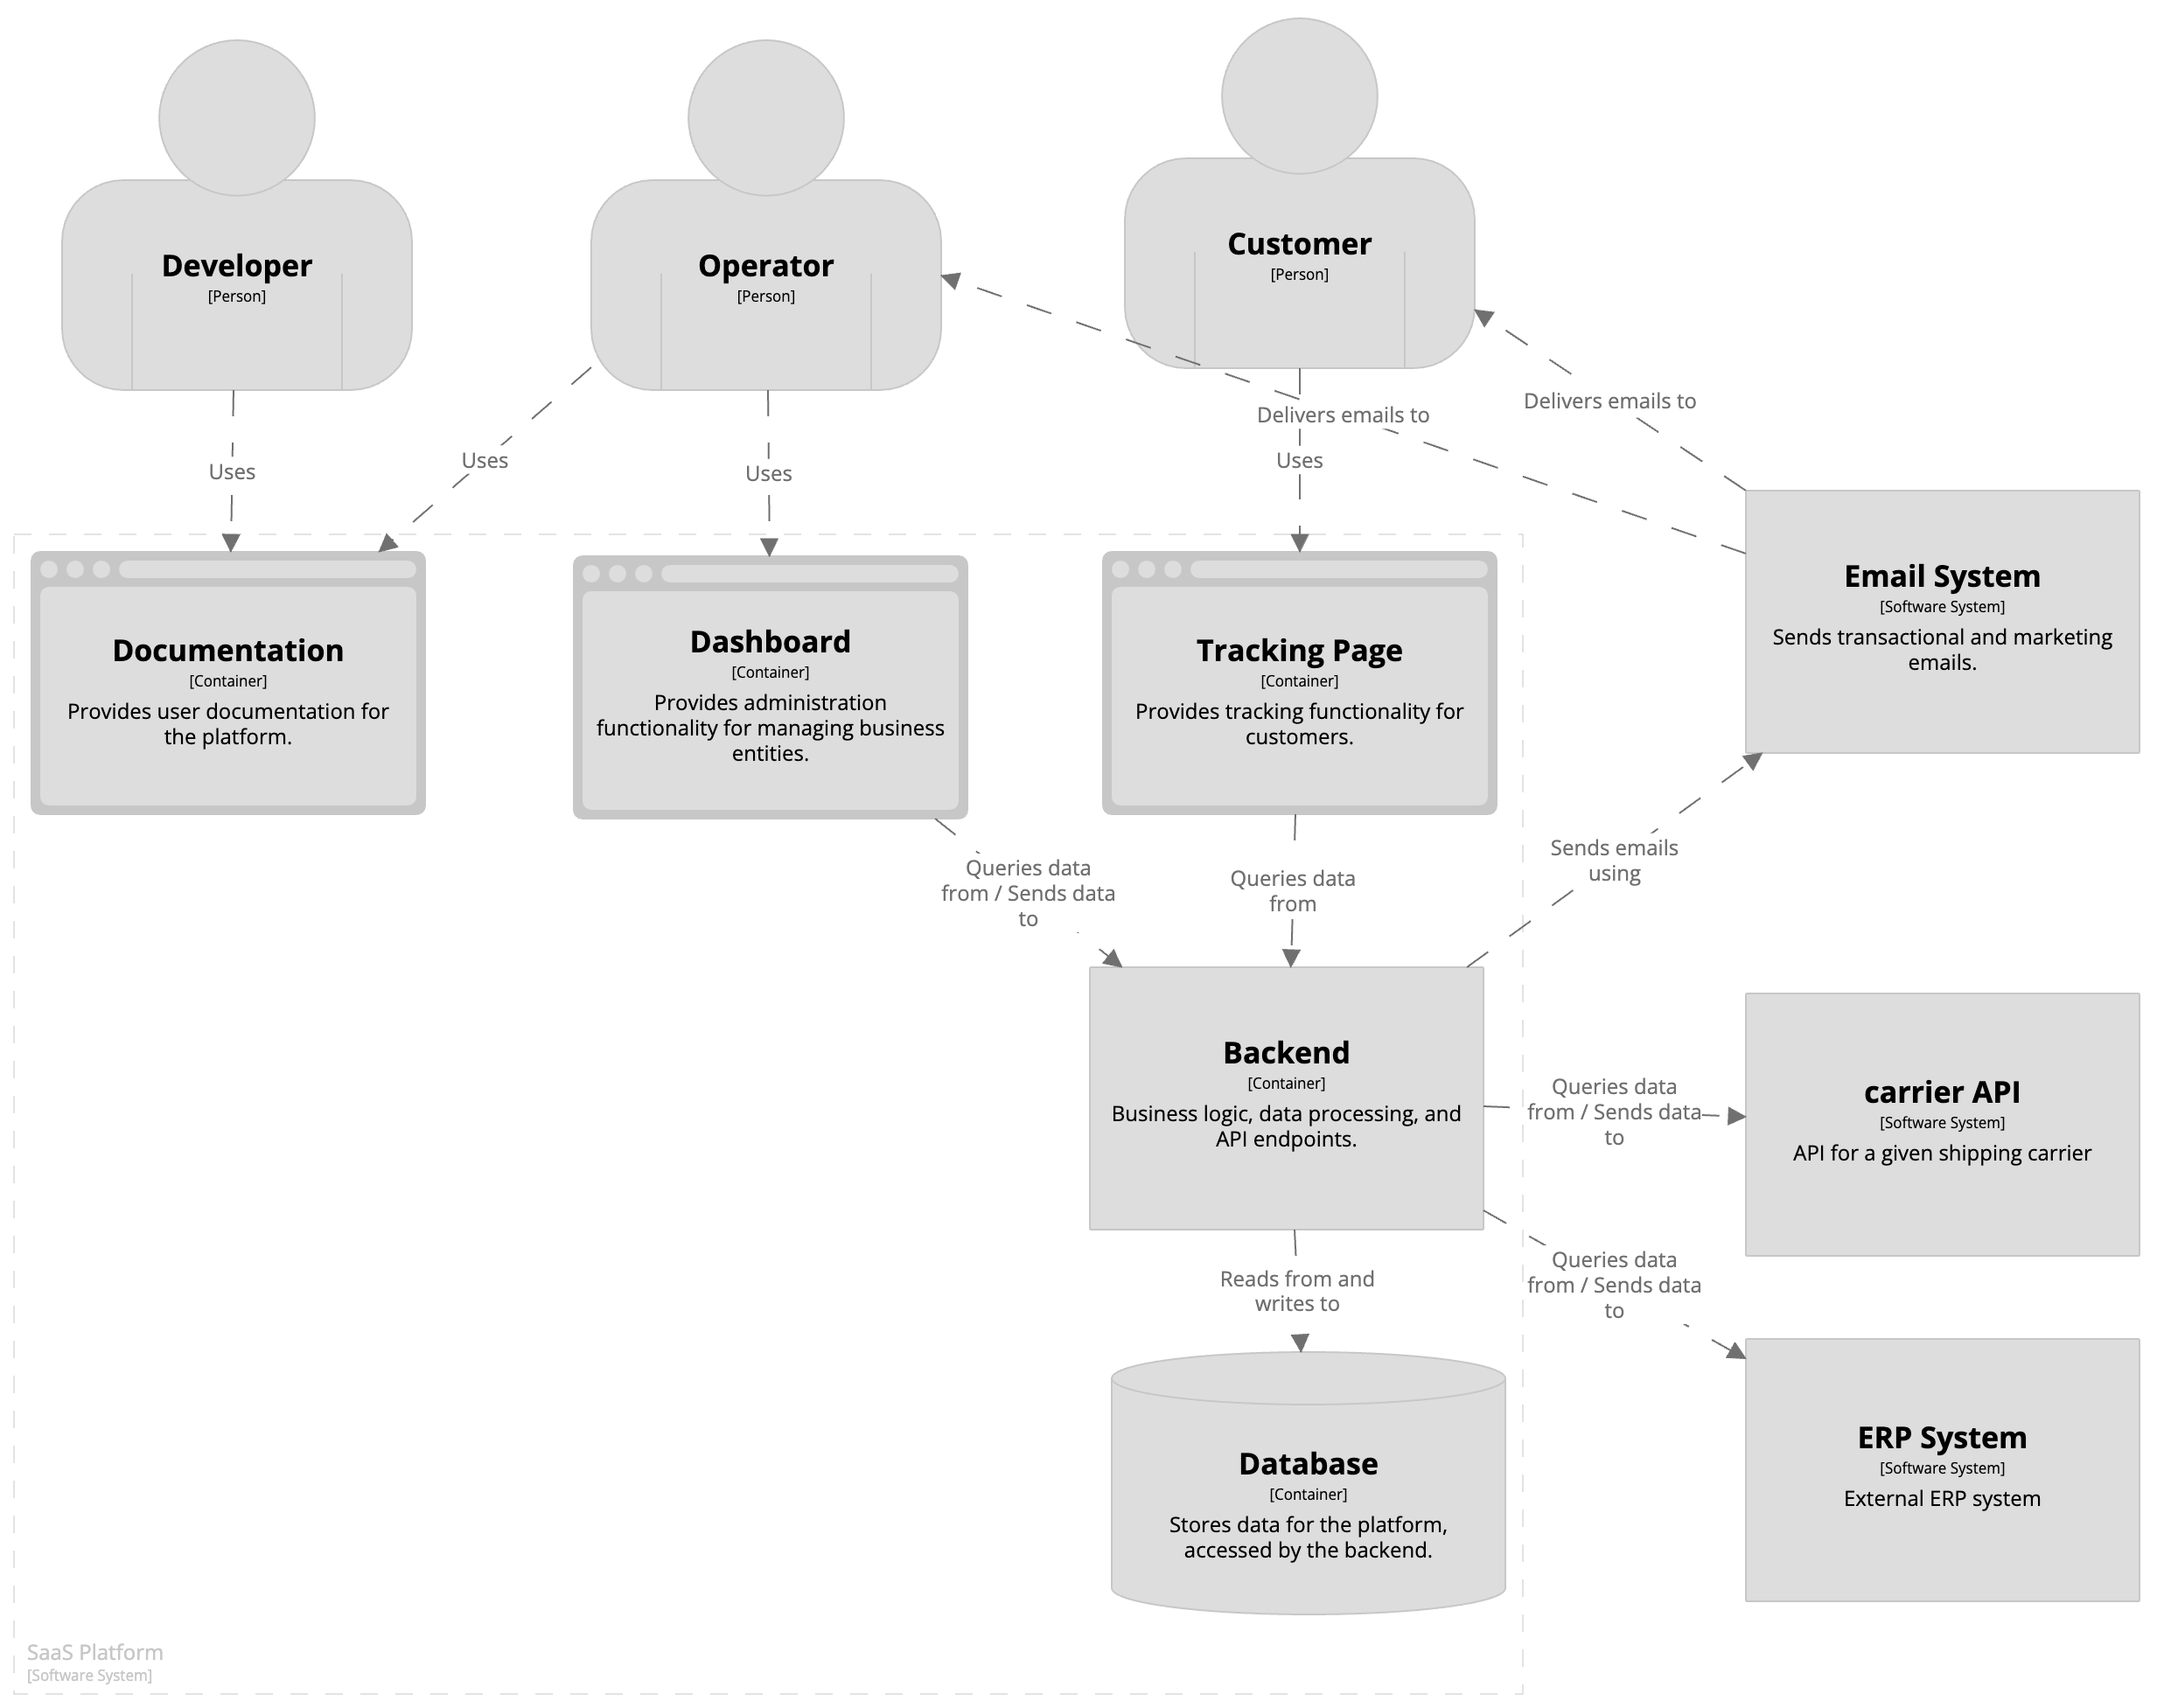
\includegraphics[width=140mm]{img/chap03/fig_architecture.png}
\caption{C4 container diagram of the software system}
\label{img03:c4_container_diagram_software_sytem}
\end{figure}

\subsection{Backend}
\label{subsec:backend}
% backend design descripiton - backend architecture in detail, including technologies used, server configurations, API design, and integration strategies
At the heart of the platform is a backend component designed to provide business logic, data processing and external communication.
The backend is structured to efficiently provide and share functionality within the component or through a set of REST API methods intended either for an internal integration of frontend components or external integrations to third-party systems.
Without diving into implementation details, the backend is designed in a way that allows it to run in a serverless environment.
The backend serves as the exclusive component directly connected to the database, making it the singular source for all \ac{CRUD} operations.
This design decision not only simplifies data management but also reinforces the security and integrity of the database.

\subsubsection{External carrier integrations}
An essential feature of backend is its capability to integrate with different shipping carriers.
This feature enables data transfer between carrier and platform, as well as label and waybill generation.
\begin{itemize}
    \item \textbf{Modular integration design:} Carrier integrations are implemented as modular components within the backend without impacting the core system.
    \item \textbf{Unified interface:} Despite the diversity of carrier APIs, the backend should abstract these differences, presenting a unified interface to the rest of the platform. This significantly simplifies the process of adding new carriers and maintaining existing ones.
    \item \textbf{Data unification:} The backend is responsible for unification of data across different carriers, translating tracking statuses into a standardised format used throughout the platform.
\end{itemize}

\subsubsection{Scheduled tasks}
To support operations that require periodic execution, such as synchronising shipment statuses or triggering the sending of email status, the backend includes a mechanism for creating scheduled tasks in a serverless environment.

\subsubsection{Public API}
A key feature of the backend is its publicly exposed Public REST API that offers a gateway for third-party integrations.
The API is documented in the OpenAPI specification.
This API facilitates secure and efficient communication. 

\subsection{Frontend}
\label{subsec:frontend}
% frontend design descripiton - frontend architecture, focusing on the user interface design, frontend frameworks, and how it interacts with the backend.
\subsubsection{Dashboard}
\subsubsection{Tracking page}
\subsection{Database}
\label{subsec:database}
 % database architecture, including the database model
\subsubsection{Data Model}
\label{subsubsec:data-model}
% in-depth look at the data model used in the project, relationship diagrams, data, and explanations of how data modeling supports the application's functionality

\chapter{Implementation}
\label{chap:implementation}

\section{Project Structure}
\label{sec:project-structure}

\subsection{Monorepo and it's advantages}
\label{subsec:monorepo-advantages}
% Detail the specific advantages of using a monorepo for this project, such as simplified dependency management, streamlined workflows, and easier code sharing between different parts of the project.

\section{API Service (Backend) Implementation}
\label{sec:api-service-implementation}
% Dedicate this section to the API service part of the project, which is built using KoaJS.

\subsection{KoaJS Framework}
\label{subsec:koajs-framework}
% brief discussion the koajs and why it was chosen for the API service. Include details on its features, benefits, and how it supports the project requirements, such as handling HTTP requests and middleware management.
% reference to the analysis

% ...

\subsection{API Design and Endpoints}
\label{subsec:api-design-endpoints}
% Discuss the design of the API, including the structure of endpoints, RESTful principles applied, and any particular design patterns or practices used.

\section{Web Client Implementation}
\label{sec:web-client-implementation}
% This section should focus on the implementation of the web client, developed using ReactJS.

\subsection{ReactJS Framework}
\label{subsec:reactjs-framework}
% Highlight its features, such as component-based architecture, and how it facilitates the development of interactive user interfaces.
% reference to the analysis

\subsection{Client-Side Routing and State Management}
\label{subsec:client-side-routing-state}
% Elaborate on the implementation of client-side routing, state management, and any other significant aspects of the web client application.

\section{Infrastructure as Code}
\label{sec:infrastructure-as-code}
%  Infrastructure as Code aspect of the project, detailing how it is integrated and managed within the monorepo.

\subsection{IaC Tools and Configuration}
\label{subsec:iac-tools-configuration}
% the tools and technologies used for IaC (Serverless), and how they are configured and utilized within the project.


\chapter{Deployment}
\label{chap:deployment}
% brief introduction into the chapter 
\section{Current Deployment Strategy}
\label{sec:current-deployment-strategy}
%  introduce the current deployment strategy of project
%  the deployment is managed using Infrastructure as Code (IaC) on AWS, use of specific services (Amazon S3 for hosting the static frontend and AWS Lambda for the backend functionality)
% how these components are organized into multiple stacks using AWS cloudformation

\subsection{Amazon S3 for Static Frontend Hosting}
\label{subsec:amazon-s3-static-frontend}
% how Amazon S3 is used for storing and serving the static ReactJS app

\subsection{AWS Lambda for Backend Services}
\label{subsec:aws-lambda-backend}
% use of AWS Lambda for the backend
% discussing how serverless architecture benefits the application, including scalability, cost-efficiency, and reduced operational overhead.

\subsection{AWS CloudFormation for Infrastructure Management}
\label{subsec:aws-cloudformation-infrastructure}
% the role of AWS cloudformation in managing the infrastructure.
% consistent, repeatable deployment processes

\section{Alternative Deployment Methods}
\label{sec:alternative-deployment-methods}
% This section should explore alternative deployment methods that could be used for the project. 

\subsection{Containerization}
\label{subsec:containerization}
% concept of containerization, particularly using Docker
% how containerization could be applied to both the frontend and backend

\subsection{Other Cloud Providers and Services}
\label{subsec:other-cloud-providers}
% Briefly touching on alternative cloud providers (like Azure or Google Cloud Platform) and their services that could be used for a similar deployment strategy.

\section{Continuous Integration and Continuous Deployment (CI/CD)}
\label{sec:cicd}
% Dedicate this section to the CI/CD processes implemented in the project, emphasizing the use of GitHub Actions.

\subsection{GitHub Actions for CI/CD}
\label{subsec:github-actions-cicd}
% how GitHub Actions are used for CI/CD
% details on how code changes in the repository trigger automated workflows for building, and deploying both the frontend and backend components

\subsection{Workflow Automation and Pipeline}
\label{subsec:workflow-automation-pipeline}
% specific steps involved in  CICD pipeline, including code commits, automated testing, build processes, and deployment to AWS services.

\chapter{Integrating SAP Business One}
\label{chap:integrating-sap-b1}

% problem description -> for the proof of context and real life texting was neccessary to build direct connection with SAP B1
% Communication with SAP isn't straight forward and is forbidden to write into SAP tables
% the decision was that the external software will be in charge of the synchronizations (call Parcelsync directly when needed, no webhooks or calls from the Parcelsync)

\section{Existing solutions}
\label{sec:existing-solutions}
% describe state of the art
\subsection{SAP Business One DI API}
\label{subsec:sap-b1-di-api}
% low level approach with direct access to the object
% was implemented in the bachaleor's thesis however did not fullfill the expectations and was pretty much phased out in favor of the SAP Business One Service Layer
\subsection{SAP Business One Service Layer}
\label{subsec:sap-b1-service-layer}
% Year after finishing the bachaleor's thesis, company moved to the newer version of SAP Business One (v9) which introduced SAP Business One Service Layer which finally brought simple REST-based approach for communicating with SAP with all mappings onto SAP objects and tables
\section{SAP Business One Service Layer Proxy with Database connector}
\label{sec:sap-b1-service-layer-proxy}
% description of the SAP Business One Server Layer Proxy which was created so that company can simply integrate Parcelsync. 
\subsection{Analysis}
\label{subsec:analysis}
% analysis of the proxy
\subsubsection{Functional requirements}
\label{subsubs:functional-requirements}
% func requirements of the proxy -> 
% - simpler authentication with basic role based access
% - proxy requests to the Service Layer
% - create database GETTER (for MS SQL DB with ODBC connector)
\subsubsection{Nonfunctional requirements}
\label{subsubsec:nonfunctional-requirements}
% deployment locally to the SAP B1 instance
% CI/CD
\subsection{Architecture}
\label{subsec:architecture}
% high level architecture of the proxy software
\subsection{Implementation}
\label{subsec:implementation}
% KoaJS app simmilar to the Parcelsync backend
\subsection{Deployment}
\label{subsec:deployment}
% Deployed as an containarized application into Docker
% Had to be local to the SAP B1 instance -> Linux VM on the server of company 


% TODO

\chapter{Testing}
\label{chap:testing}

\section{Environments}
\label{sec:environments}
% local, staging, production
\subsection{Local}
\label{subsec:local}
% serverless-offline
% docker database
\subsection{Staging, Production}
\label{subsec:staging-production}
% on the AWS

\section{Testing the GUI}
\label{sec:testing-gui}
\section{}
\chapter*{Conclusion}
\addcontentsline{toc}{chapter}{Conclusion}


%%% Bibliography
%%% Bibliography (literature used as a source)
%%%
%%% We employ bibTeX to construct the bibliography. It processes
%%% citations in the text (e.g., the \cite{...} macro) and looks up
%%% relevant entries in the bibliography.bib file.
%%%
%%% The \bibliographystyle command selects, which style will be used
%%% for references from the text. The argument in curly brackets is
%%% the name of the corresponding style file (*.bst). Both styles
%%% mentioned in this template are included in LaTeX distributions.

\bibliographystyle{plainnat}    %% Author (year)
% \bibliographystyle{unsrt}     %% [number]

\renewcommand{\bibname}{Bibliography}

%%% Generate the bibliography. Beware that if you cited no works,
%%% the empty list will be omitted completely.

\bibliography{bibliography}

%%% If case you prefer to write the bibliography manually (without bibTeX),
%%% you can use the following. Please follow the ISO 690 standard and
%%% citation conventions of your field of research.

% \begin{thebibliography}{99}
%
% \bibitem{lamport94}
%   {\sc Lamport,} Leslie.
%   \emph{\LaTeX: A Document Preparation System}.
%   2nd edition.
%   Massachusetts: Addison Wesley, 1994.
%   ISBN 0-201-52983-1.
%
% \end{thebibliography}


%%% Figures used in the thesis (consider if this is needed)
\listoffigures

%%% Tables used in the thesis (consider if this is needed)
%%% In mathematical theses, it could be better to move the list of tables to the beginning of the thesis.
\listoftables

%%% Abbreviations used in the thesis, if any, including their explanation
%%% In mathematical theses, it could be better to move the list of abbreviations to the beginning of the thesis.
\chapwithtoc{List of Abbreviations}

%%% Attachments to the master thesis, if any. Each attachment must be
%%% referred to at least once from the text of the thesis. Attachments
%%% are numbered.
%%%
%%% The printed version should preferably contain attachments, which can be
%%% read (additional tables and charts, supplementary text, examples of
%%% program output, etc.). The electronic version is more suited for attachments
%%% which will likely be used in an electronic form rather than read (program
%%% source code, data files, interactive charts, etc.). Electronic attachments
%%% should be uploaded to SIS and optionally also included in the thesis on a~CD/DVD.
%%% Allowed file formats are specified in provision of the rector no. 72/2017.
\appendix
\chapter{Attachments}

\section{First Attachment}

\openright
\end{document}
